\chapter{Повышение резкости медицинских изображений методом деформации пиксельной сетки}\label{ch:ch2}

На практике часто возникает необходимость повышения резкости изображений по разным причинам: из-за физических ограничений оптических систем и сенсоров камер или из-за сложных условий получения изображений. В то же время в медицине при обработке изображений важно не терять присутствующие на них детали или добавлять не существовавшие элементы или артефакты.

В отличие от наиболее распространённых методов повышения резкости (обращение свёртки, нерезкое маскирование), деформационный метод, представленный в~\cite{krylov2014gridwarping} и затем доработанный в~\cite{nasonova2014deblurred, gusev2016parallel}, не меняет значения интенсивности пикселей, а сдвигает сами пиксели в окрестности контуров изображений~(см.~Рис~\ref{fig:warping-warping-idea}). Этот подход изменяет изображение в окрестности контуров и не имеет таких недостатков, свойственных некоторым другим методам, как усиление шума и возникновение эффекта ложного оконтуривания.

\begin{figure}[ht]
	\centerfloat{
		\hfill
		\subcaptionbox[List-of-Figures entry]{Профиль контура}{%
			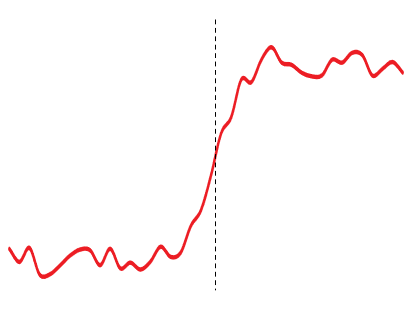
\includegraphics[width=0.3\textwidth]{warping-1-4b.png}}
		\hfill
		\subcaptionbox{Классический метод}{%
			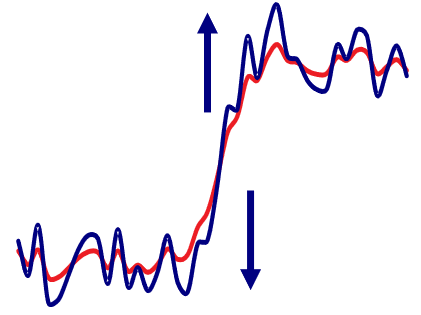
\includegraphics[width=0.3\textwidth]{warping-1-4a.png}}
		\hfill
		\subcaptionbox{Деформационный метод}{%
			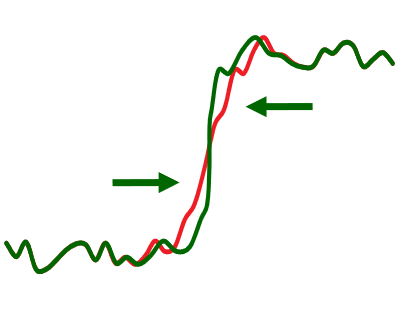
\includegraphics[width=0.3\textwidth]{warping-1-4c.png}}
		\hfill
	}
	\caption{Принцип работы классических методов и деформационного метода повышения резкости изображений}
	\label{fig:warping-warping-idea}
\end{figure}

В данной главе рассматривается деформационный алгоритм повышения резкости изображения~\cite{nasonova2014deblurred, gusev2016parallel} и набор из 24 тестовых изображений из базы TID2013~\cite{ponomarenko2015image}, размытых с разной интенсивностью с использованием трёх типов реалистичных ядер размытия. Целью является нахождение оптимальной функции смещения для каждого типа ядра размытия отдельно и для всех типов сразу.

\section{Реалистичные ядра размытия изображений}

Модель размытия изображения, рассматриваемая в этой главе, совпадает с моделью, описанной в п.~\ref{sec:image-blur-model}.

В данной работе рассматриваются три типа ядер размытия, возникающих на практике: ядро, определяемое функцией Гаусса; и два ядра, которые часто возникают в реальных изображения, полученных с помощью фотокамер.

Ядро Гаусса выбрано по той причине, что оно соответствует одной из наиболее распространённых моделей размытия изображения, а также потому, что такое ядро (или очень близкое к нему) можно встретить в изображениях, полученных с помощью некоторых оптических систем, где дифракция света играет заметную роль (например, с помощью микроскопов).

Также, согласно модели Зейделя, существует пять видов оптических аберраций~\cite{simpkins2014parameterized}:

\begin{enumerate}
	\item сферическая аберрация;
	\item кома;
	\item астигматизм;
	\item кривизна поля изображения;
	\item дисторсия.
\end{enumerate}

Ядра, отвечающие сферическим аберрациям и астигматизму, также схожи с ядром Гаусса~\cite{simpkins2014parameterized, simpkins2011modeling}, что послужило дополнительным аргументом в пользу рассмотрения этого ядра. Примеры этих искажений представлены на Рис.~\ref{fig:warping-aberrations})

\begin{figure}[ht]
	\centerfloat{
		\hfill
		\subcaptionbox[List-of-Figures entry]{Сферическая аберрация}{%
			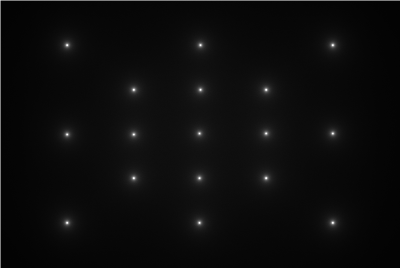
\includegraphics[width=0.45\textwidth]{warping-1-1a.png}}
		\hfill
		\subcaptionbox{Кома}{%
			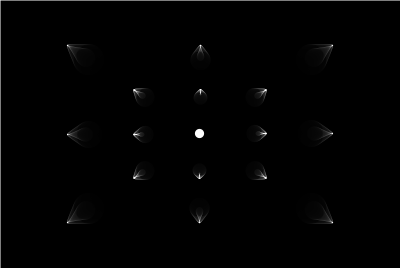
\includegraphics[width=0.45\textwidth]{warping-1-1b.png}}
		\hfill
		\vfill
		\hfill
		\subcaptionbox{Астигматизм}{%
			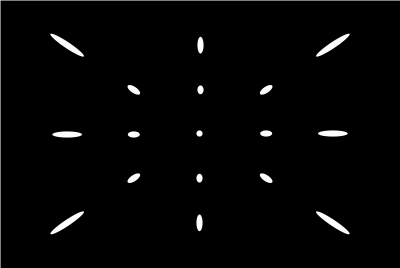
\includegraphics[width=0.45\textwidth]{warping-1-1c.png}}
		\hfill
		\subcaptionbox{Разные виды астигматизма}{%
			
\includegraphics[width=0.45\textwidth]{warping-1-1d.png}}
		\hfill
		\vfill
		\hfill
		\subcaptionbox{Кривизна поля изображения}{%
			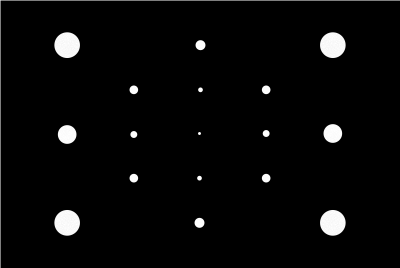
\includegraphics[width=0.45\textwidth]{warping-1-1e.png}}
		\hfill
		\subcaptionbox{Дисторсия}{%
			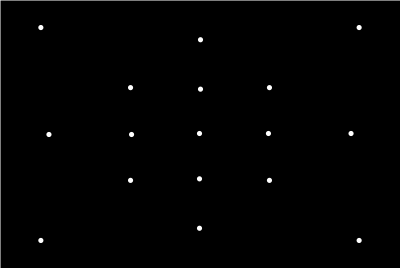
\includegraphics[width=0.45\textwidth]{warping-1-1f.png}}
		\hfill
		\vfill
	}
	\caption{Виды оптический аберраций}
	\label{fig:warping-aberrations}
\end{figure}

Помимо этих пяти аберраций также встречаются просто расфокусированные изображения, либо же расфокусированные участки изображений, полученных с использованием камер с малой глубиной резкости изображаемого пространства. В таком случае полученное изображение точки имеет вид круга с приблизительно равномерной яркостью, однако также может иметь увеличение яркости в центре или на краях (что выглядит как круг с кольцом). Таким образом, ядро размытия часто имеет вид круга или круга с кольцом. Конкретный вид зависит в том числе от положения объекта на изображении относительно области, находящейся  в фокусе. Примеры этого эффекта приведены на Рис.~\ref{fig:warping-defocus}.

\begin{figure}[ht]
	\centerfloat{
		\hfill
%		\subcaptionbox[List-of-Figures entry]{Объект за областью резкости}{%
%			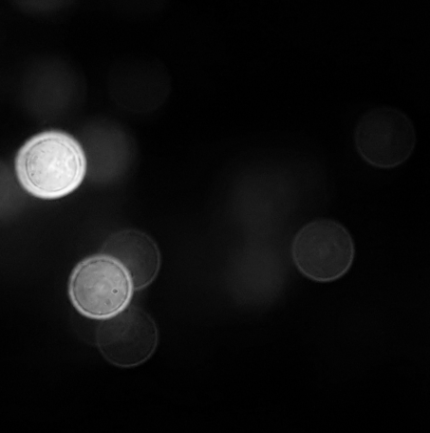
\includegraphics[width=0.25\textwidth]{warping-1-2a.png}}
%		\hfill
		\subcaptionbox{Объект за областью резкости}{%
			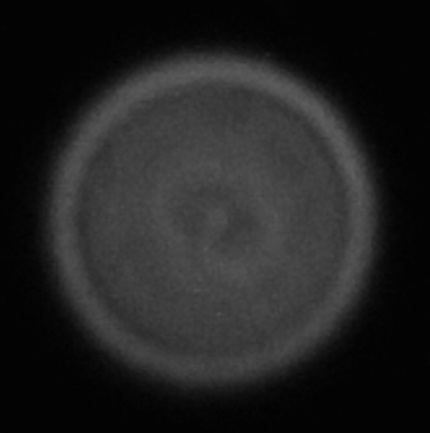
\includegraphics[width=0.25\textwidth]{warping-1-2b.png}}
		\hfill
		\subcaptionbox{Объект перед областью резкости}{%
			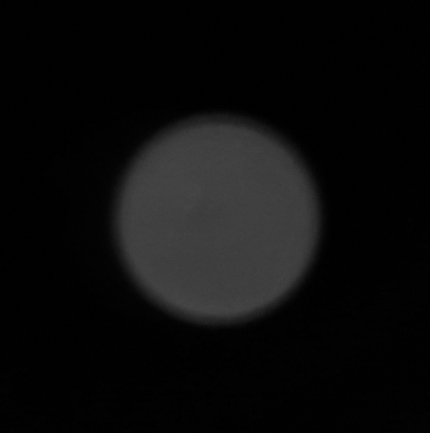
\includegraphics[width=0.25\textwidth]{warping-1-2c.png}}
		\hfill
	}
	\caption{Примеры эффекта расфокусировки}
	\label{fig:warping-defocus}
\end{figure}

Итак, модели ядер, рассматриваемые в данной работе, это:

\begin{enumerate}
	\item Ядро Гаусса.
	Задаётся формулой $f\left(x\right)=\frac{1}{2\pi\sigma^2}e^{-\frac{x^2+y^2}{2\sigma^2}}$. Радиусом этого ядра будет считаться величина $3\sigma$.
	\item Круг.
	Постоянное положительное значение в пределах круга, вне круга нуль. Радиус ядра "--- радиус круга.
	\item Круг с кольцом.
	Постоянное положительное значение внутри круга и значение, на 33\% большее, на его границе (на расстоянии 0.85 радиуса от центра и дальше). Радиус ядра "--- радиус самого круга.
\end{enumerate}

Примеры этих ядер представлены на Рис.~\ref{fig:warping-psf-examples}. 

\begin{figure}[ht]
	\centerfloat{
		\hfill
		\subcaptionbox[List-of-Figures entry]{Гауссово ядро (Г)}{%
			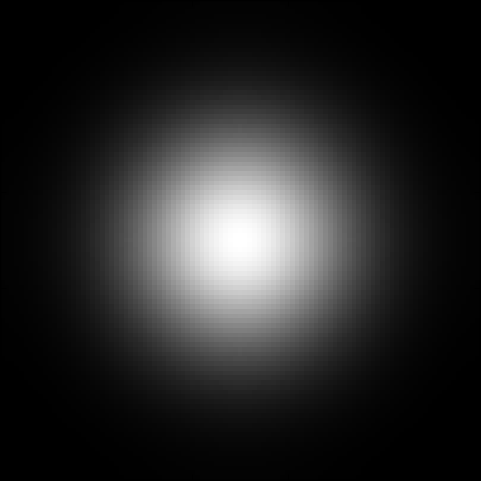
\includegraphics[width=0.25\textwidth]{warping-1-3a.png}}
		\hfill
		\subcaptionbox{Круг (К)}{%
			
\includegraphics[width=0.25\textwidth]{warping-1-3b.png}}
		\hfill
		\subcaptionbox{Круг с кольцом (КЦ)}{%
			
\includegraphics[width=0.25\textwidth]{warping-1-3c.png}}
		\hfill
	}
	\caption{Рассматриваемые ядра размытия}
	\label{fig:warping-psf-examples}
\end{figure}

\section{Построение тестового набора изображений}

В работе использовался набор из 24 естественных изображений из базы TID2008~\cite{ponomarenko2009tid2008}, которая является одним из стандартных наборов данных для тестирования методов обработки изображений.

При построении тестового набора к каждому изображению применялся оператор свёртки с каждым из трёх ядер размытия с разным радиусом ядра. Для круга и круга с кольцом радиус ядра размытия изменялся в пределах от 1.5 до 5 пикселей с шагом 0.5 пикселя. Для гауссова ядра "--- в пределах от 2.25 до 7.5 с шагом 0.75, что соответствует изменениям параметра $\sigma$ в пределах от 0.75 до 2.5 с шагом 0.25.

В результате для каждого типа размытия был сформирован набор из 192 изображений.

\section{Деформационный метод повышения резкости изображений}

В процессе работы алгоритма на изображении:

\begin{enumerate}
	\item обнаруживаются контуры алгоритмом Кэнни~\cite{canny1986computational},
	\item производится расчёт векторов смещения пикселей в окрестности контуров,
	\item в соответствии с вычисленным векторным полем смещений деформируется пиксельная сетка,
	\item полученный результат проецируется на регулярную сетку выходного изображения с помощью интерполяции, описанной в~\cite{krylov2014gridwarping}.
\end{enumerate}

Направление и величина смещения пикселей задаётся функцией смещения $d\left(x\right)$, $x_{new} \leftarrow x_{old}+d(x_{old})$. В одномерном случае, если центр контура находится в точке $x = 0$, вектора смещения определяются функцией близости $p\left(x\right)=1+d^{\,\prime}(x)$.

Она может быть выражена через p(x) с помощью уравнения

\begin{equation*}
	d\left(x\right)=\int_{-\infty}^{x}\left(p\left(y\right)-1\right)dy.
\end{equation*}

Функция $p(x)$ выражает расстояние между соседними пикселями изображения: если её значение меньше 1, в точке $x$ уплотнение; если больше 1 "--- разрежение. Для недеформированных изображений $p(x)\equiv1$.
Чтобы взаимное расположение точек при смещении не менялось, для функции $d(x)$ должно быть выполнено $x_1<x_2 \Rightarrow x_1+d(x_1)\le x_2+d(x_2)$. Отсюда получаем ограничение $d^{\,\prime}\left(x\right)\geq-1$. Также деформироваться должна только сетка вблизи контуров, поэтому $d\left(x\right)\rightarrow0$ при  $\left|x\right|\rightarrow\infty$. Пример функции близости приведён на Рис.~\ref{fig:warping-proximity}.

\begin{figure}[ht]
	\centerfloat{
		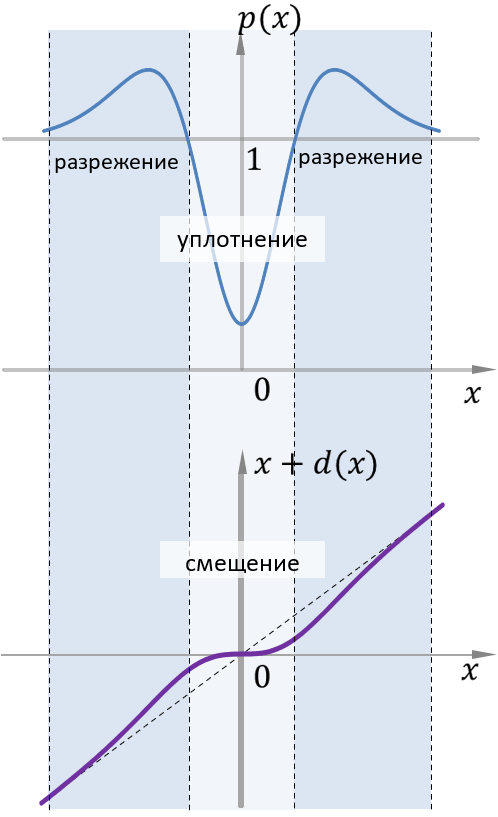
\includegraphics[height=0.4\textheight]{warping-1-5.png}
	}
	\caption{Пример функции близости и результата смещения пикселей с её помощью}
	\label{fig:warping-proximity}
\end{figure}

В двумерном случае смещение задаётся векторным полем $\vec{d}(x,y)$, которое удовлетворяет уравнению $p\left(x,y\right)=1+div\vec{d}(x,y)$.
Если функция $p(x, y)$ известна, то $\vec{d}(x,y)$ находится решением уравнения $\vec{d}\left(x,y\right)=\nabla u\left(x,y\right)$.

Помимо этого во избежание возникновения завихрений требуется ограничение $rot \vec{d}=0$, а так как $rot \nabla u \equiv 0$, то векторное поле смещений можно представить как $\nabla u(x,y)$, где функция $u(x,y)$ является решением уравнения

\begin{equation*}
	\left\{
		\begin{aligned}
			&\Delta u = p(x,y) - 1, \\
			&u\mid_\Gamma=0,
		\end{aligned}
	\right.
\end{equation*}

\noindent где $\Gamma$ "--- граница изображения.

В работе~\cite{gusev2016parallel} предлагается для двумерного случая использовать функцию близости одной переменной для построения функции близости на плоскости:

\begin{align*}
	&p\left(x,y\right) = \frac{\sum_{\left(x_e,y_e\right) \in N\left(x,y\right)}{w\left(x_e,y_e\right)p\left(x_n\right)}} {\sum_{\left(x_e,y_e\right) \in N\left(x,y\right)}{w\left(x_e,y_e\right)}},
	&G_{\sigma}\left(x_t\right)\lvert \vec{g}\left(x_e,y_e\right) \rvert,
\end{align*}

\noindent где $N\left(x,y\right)$ "--- это множество соседних точек вокруг т.~$\left(x, y\right)$; $x_n$ и $x_t$ "--- это проекции вектора $\left(x-x_e, y-y_e\right)$ на вектор градиента изображения $\vec{g}\left(x_e,y_e\right)$ и на нормаль к нему соответственно; а $G_{\sigma}\left(x_t\right) = \frac{1}{\sigma \sqrt{2\pi}} \exp\left(\frac{-x^2}{2\sigma^2}\right)$.

В этом случае итоговая функция смещения имеет следующий вид~\cite{gusev2016parallel}:

\begin{equation*}
	\vec{d}\left(x,y\right) = \frac{\sum_{\left(x_e,y_e\right) \in N\left(x,y\right)}{d\left(x_n\right) G_{\sigma}\left(x_t\right) \vec{g}\left(x_e,y_e\right) }} {\sum_{\left(x_e,y_e\right) \in N\left(x,y\right)}{G_{\sigma}\left(x_t\right)\lvert \vec{g}\left(x_e,y_e\right) \rvert}}.
\end{equation*}

Таким образом, можно перейти к работе с функцией смещения напрямую и проанализировать её влияние на результаты работы деформационного алгоритма повышения резкости.

\section{Модели функции смещения}

В работе рассматриваются три модели функции смещения, первая из которых была предложена в оригинальной работе авторов метода:

\begin{enumerate}
	\item $d_0\left(x;\sigma\right)=\sigma\sqrt\pi\left[erf\left(\frac{x}{2\sigma}\right)-erf\left(\frac{x}{\sigma}\right)\right]$, где $erf{\left(x\right)}=\frac{2}{\sqrt\pi}\int_{0}^{x}{e^{-t^2}dt}$;
	\item
	$
	\begin{aligned}
		d_2\left(x;a,b,c\right)=\left\{
		\begin{aligned}
			&\frac{c}{a}x,\ \left|x\right|<a,\\
			&c\frac{b-\left|x\right|}{b-a} \cdot sign\left(x\right),\ a\le\left|x\right|<b,\\
			&0,\ \left|x\right|\geq b;
		\end{aligned}
		\right.
	\end{aligned}
	$
	\item $d_1(x;a,c)$, имеющая тот же вид, что и $d_2(x)$, но $b=1.5a$.
\end{enumerate}

При этом параметры $a$, $b$ и $c$ пропорциональны радиусу ядра размытия, что позволяет масштабировать функцию для разных уровней размытия. Для функции $d_0\left(x;\sigma\right)$ тот же эффект достигается с помощью параметра $\sigma$.

Пример функции $d_2(x;a,b,c)$ приведёт на Рис.~\ref{fig:warping-d2-example}.

\begin{figure}[ht]
	\centerfloat{
		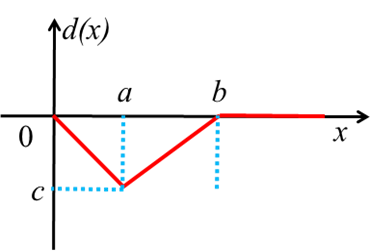
\includegraphics[width=0.4\textwidth]{warping-1-6.png}
	}
	\caption{Вид функции смещения $d_2(x;a,b,c)$}
	\label{fig:warping-d2-example}
\end{figure}

\section{Методика тестирования моделей функций смещения}

Проводился поиск оптимальных параметров рассматриваемых моделей функций смещения для разных типов размытия, а затем "--- сравнительный анализ результатов обработки размытых изображений деформационным методом повышения резкости с использованием полученных результатов.

Для нахождения оптимальных параметров проводилась минимизация среднего значения метрики RMSE по всем изображениям для одного типа размытия:

\begin{align*}
	&\frac{1}{\left|V\right|}\sum_{V}{RMSE(u,v)\rightarrow \min_{z}},
	&RMSE\left(u,v\right)=\sqrt{\frac{1}{WH}\sum_{i,j}{(u_{ij}-v_{ij})}^2}.
\end{align*}

Здесь $v$ "--- размытое изображение, обработанное методом повышения резкости, $u$ "--- соответствующее ему истинное резкое изображение, $V$ "--- множество всех размытых изображений для одного ядра размытия, $W$ и $H$ "--- ширина и высота изображения в пикселях соответственно, $z$ "--- соответствующие рассматриваемой функции смещения параметры из множества $\left\{a, b, c\right\}$.

Для решения задачи минимизации применялся метод Нелдера"=Мида~\cite{10.1093/comjnl/7.4.308}. Несмотря на то, что метод обнаруживает локальные минимумы, применение этого алгоритма с разными начальными приближениями во всех случаях приводило к одинаковым результатам.

\section{Результаты сравнения моделей функций смещения}

В ходе экспериментов было установлено, что наилучшие результаты достигаются при $a=-c$. Такое соотношение параметров обеспечивает наибольшее смещение пикселей в районе контура без нарушения ограничения на производную функции смещения. Поэтому в дальнейшем это соотношение всегда выполняется, что позволяет перейти к модели с двумя (функция $d_2(x;a,b,c=-a)$) и одним (функция $d_1(x;a,c=-a)$) параметрами.

После проведения исследования и поиска оптимальных параметров функций смещения для каждого типа размытия были получены следующие результаты.

На Рис.~\ref{fig:warping-best-displacements} представлены функции смещения, оптимальные только для своего типа размытия, после нормировки параметров на радиус размытия. Красным цветом отмечена модель с двумя параметрами (c функцией $d_2\left(x\right)$), а синим "--- модель с одним параметром  (c функцией $d_1\left(x\right)$). Условные обозначения типов ядер размытия: К "--- круг, КЦ "--- круг с кольцом, Г "--- гауссово ядро.

\begin{figure}[ht]
	\centerfloat{
		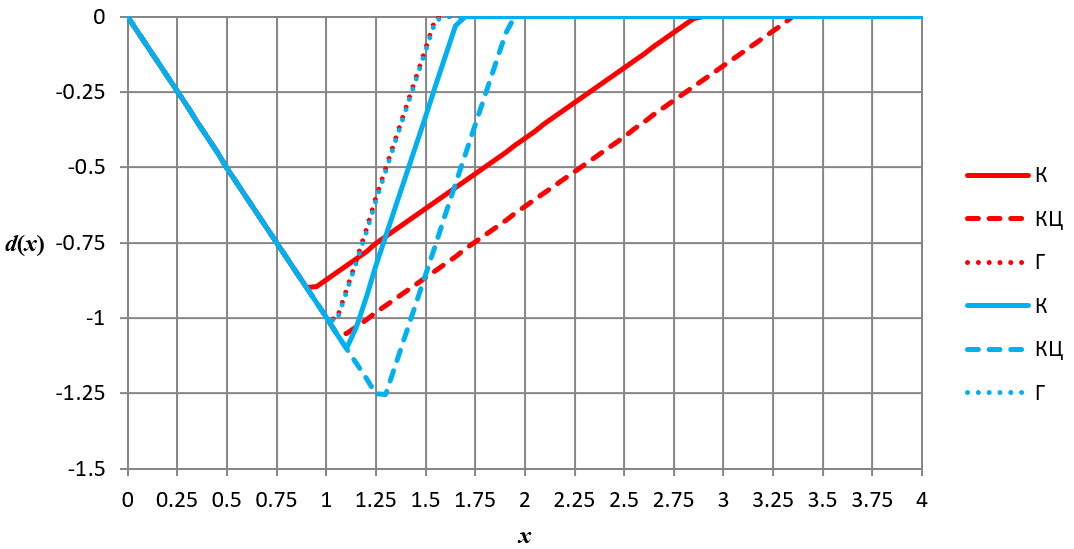
\includegraphics[width=0.9\textwidth]{warping-1-7.png}
	}
	\caption{Функция смещения для моделей с 1 и 2 параметрами}
	\label{fig:warping-best-displacements}
\end{figure}

Усреднённые по набору изображений значения RMSE входных размытых и обработанных изображений для функций смещения $d_0\left(x\right)$ и $d_2\left(x\right)$ с оптимальными параметрами приведены в Табл.~\ref{tab:warping-rmse-d0-d2}. Из неё видно, что предложенная функция $d_2\left(x\right)$ позволяет достичь более качественного результата.

\begin{table} [htbp]%
%	\tiny
	\small
	\centering
	\caption{Средние значения RMSE размытых и обработанных изображений для функций смещения $d_0\left(x\right)$ и $d_2\left(x\right)$ (сила размытия обозначена номером радиуса размытия в порядке возрастания)}%
	\label{tab:warping-rmse-d0-d2}% label всегда желательно идти после caption
	\renewcommand{\arraystretch}{1.5}%% Увеличение расстояния между рядами, для улучшения восприятия.
	\begin{SingleSpace}
		\begin{tabulary}{\textwidth}{@{}@{\extracolsep{5pt}}cCCCCCCCCC@{}} %Вертикальные полосы не используются принципиально, как и лишние горизонтальные (допускается по ГОСТ 2.105 пункт 4.4.5) % @{} позволяет прижиматься к краям
			\toprule     %%% верхняя линейка
			& \multicolumn{3}{@{}c@{}}{\makecell{Размытые \\ изображения}} & \multicolumn{3}{@{}c@{}}{\makecell{$d_0\left(x\right)$}} & \multicolumn{3}{@{}c@{}}{\makecell{$d_2\left(x\right)$}} \\
			\cmidrule(r){2-4}\cmidrule(lr){5-7}\cmidrule(l){8-10}
			\makecell{Сила \\ размытия}  &  Г & К & КЦ  &  Г & К & КЦ  &  Г & К & КЦ \\
			\midrule %%% тонкий разделитель. Отделяет названия столбцов. Обязателен по ГОСТ 2.105 пункт 4.4.5
			1 & 13.470 & 9.750 & 11.004 & 13.119 & 9.603 & 10.794 & 13.015 & 9.516 & 10.620 \\
			2 & 15.481 & 11.849 & 13.525 & 15.039 & 11.585 & 13.176 & 14.912 & 11.492 & 12.974 \\
			3 & 16.905 & 13.869 & 15.446 & 16.385 & 13.483 & 14.980 & 16.260 & 13.365 & 14.750 \\
			4 & 18.037 & 14.975 & 16.383 & 17.489 & 14.558 & 15.898 & 17.370 & 14.455 & 15.710 \\
			5 & 18.951 & 16.093 & 17.488 & 18.386 & 15.622 & 16.954 & 18.274 & 15.525 & 16.782 \\
			6 & 19.749 & 16.893 & 18.255 & 19.169 & 16.412 & 17.712 & 19.063 & 16.327 & 17.563 \\
			7 & 20.437 & 17.625 & 18.973 & 19.836 & 17.120 & 18.405 & 19.730 & 17.044 & 18.273 \\
			8 & 21.070 & 18.270 & 19.599 & 20.462 & 17.761 & 19.027 & 20.352 & 17.693 & 18.905 \\
			\midrule
			Среднее & 18.013 & 14.916 & 16.334 & 17.486 & 14.518 & 15.868 & 17.372 & 14.427 & 15.697 \\
			\bottomrule %%% нижняя линейка
		\end{tabulary}%
	\end{SingleSpace}
\end{table}

В Табл.~\ref{tab:warping-rmse-d1} представлены показатели снижения RMSE относительно размытых изображений для вариантов алгоритма на основе функции смещения с 2 и с 1 параметром. Модуль относительной разницы не превышает 4\%, а в среднем равен 1.2\%, что позволяет говорить о сравнимом качестве работы обоих вариантов метода и возможности использовать однопараметрический вариант без значительных потерь в качестве.

\begin{table} [htbp]%
	\centering
	\caption{Средние значения снижения RMSE для изображений, обработанных с использованием функции смещения $d_2\left(x\right)$ и $d_1\left(x\right)$, по сравнению с размытыми изображениями}%
	\label{tab:warping-rmse-d1}% label всегда желательно идти после caption
	\renewcommand{\arraystretch}{1.5}%% Увеличение расстояния между рядами, для улучшения восприятия.
	\begin{SingleSpace}
		\begin{tabulary}{\textwidth}{@{}@{\extracolsep{10pt}}cCCCCCC@{}} %Вертикальные полосы не используются принципиально, как и лишние горизонтальные (допускается по ГОСТ 2.105 пункт 4.4.5) % @{} позволяет прижиматься к краям
			\toprule     %%% верхняя линейка
			& \multicolumn{3}{@{}c@{}}{\makecell{$d_2\left(x\right)$}} & \multicolumn{3}{@{}c@{}}{\makecell{$d_1\left(x\right)$}} \\
			\cmidrule(r){2-4}\cmidrule(l){5-7}
			\makecell{Сила \\ размытия}  &  Г & К & КЦ  &  Г & К & КЦ \\
			\midrule %%% тонкий разделитель. Отделяет названия столбцов. Обязателен по ГОСТ 2.105 пункт 4.4.5
			1 & 0.455 & 0.234 & 0.384 & 0.456 & 0.227 & 0.399 \\
			2 & 0.569 & 0.357 & 0.551 & 0.569 & 0.365 & 0.551 \\
			3 & 0.645 & 0.504 & 0.696 & 0.645 & 0.508 & 0.671 \\
			4 & 0.667 & 0.520 & 0.673 & 0.666 & 0.518 & 0.654 \\
			5 & 0.677 & 0.568 & 0.706 & 0.677 & 0.563 & 0.693 \\
			6 & 0.686 & 0.566 & 0.692 & 0.686 & 0.56 & 0.682 \\
			7 & 0.707 & 0.581 & 0.700 & 0.708 & 0.578 & 0.687 \\
			8 & 0.718 & 0.577 & 0.694 & 0.718 & 0.575 & 0.676 \\
			\midrule
			Среднее & 0.641 & 0.489 & 0.637 & 0.641 & 0.487 & 0.627 \\
			\bottomrule %%% нижняя линейка
		\end{tabulary}%
	\end{SingleSpace}
\end{table}

Из Рис.~\ref{fig:warping-best-displacements} видно, что для разных типов ядер размытия относительные значения оптимальных параметров функций смещения близки. Дополнительный анализ изменения среднего прироста метрики PSNR показал, что при несильном отклонении параметра от оптимального значения качество результирующего изображения снижается слабо (см. Рис.~\ref{fig:warping-isnr-change}), поэтому для всех трёх видов ядер размытия можно применять одну и ту же функцию однопараметрическую смещения, где параметр $a$ равен радиусу ядра.

\begin{figure}[ht]
	\centerfloat{
		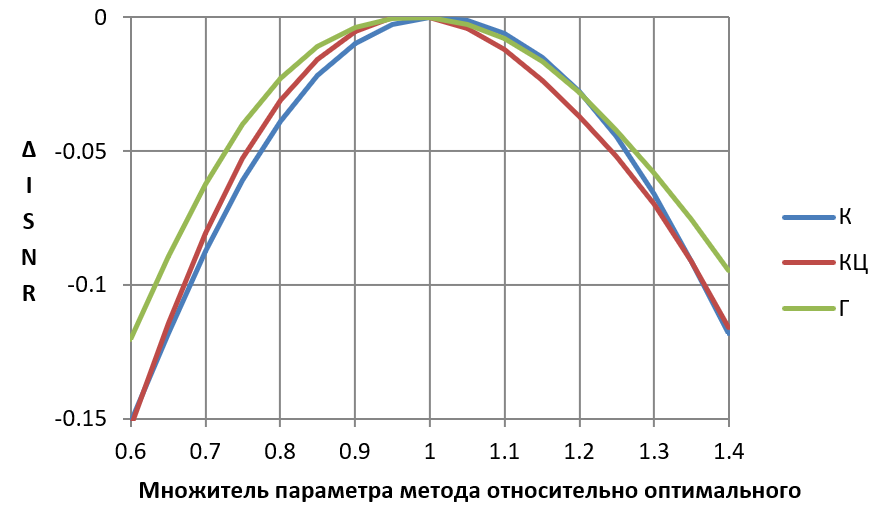
\includegraphics[width=0.8\textwidth]{warping-1-extra1.png}
	}
	\caption{Изменение прироста метрики PSNR при относительном изменении параметра $a$}
	\label{fig:warping-isnr-change}
\end{figure}

На Рис.~\ref{fig:warping-eye}~и~\ref{fig:warping-eye2} приведены примеры результата обработки медицинского изображения полученным методом. Видно повышение резкости контуров сосудов и диска зрительного нерва.

\begin{figure}[ht]
	\centerfloat{
		\hfill
		\subcaptionbox[List-of-Figures entry]{Входное изображение}{%
			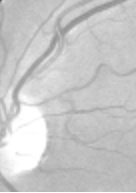
\includegraphics[height=0.3\textheight]{warping-1-8a.png}}
		\hfill
		\subcaptionbox{Обработанное изображение}{%
			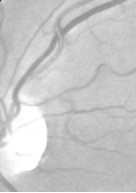
\includegraphics[height=0.3\textheight]{warping-1-8b.png}}
		\hfill
	}
	\caption{Применение деформационного алгоритма с использованием функции смещения $d_1\left(x\right)$ как шага постобработки в задаче повышения разрешения медицинских изображений}
	\label{fig:warping-eye}
\end{figure}

\begin{figure}[ht]
	\centerfloat{
		\hfill
		\subcaptionbox[List-of-Figures entry]{Входное изображение}{%
			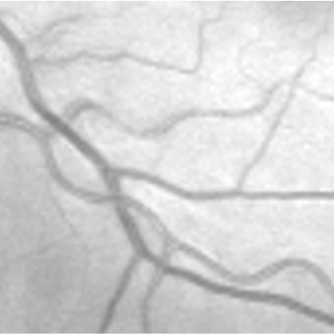
\includegraphics[height=0.25\textheight]{warping-1-extra2a.png}}
		\hfill
		\subcaptionbox{Обработанное изображение}{%
			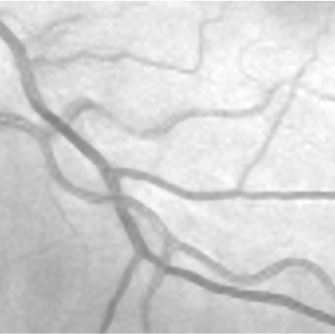
\includegraphics[height=0.25\textheight]{warping-1-extra2b.png}}
		\hfill
	}
	\caption{Применение деформационного алгоритма с использованием функции смещения $d_1\left(x\right)$ как шага постобработки в задаче повышения разрешения медицинских изображений}
	\label{fig:warping-eye2}
\end{figure}

\section{Выводы} 

Предложенные функции смещения $d_2\left(x\right)$ и $d_1\left(x\right)$ демонстрируют улучшение качества обработки изображений по сравнению с оригинальной функцией $d_0\left(x\right)$, выражаемое в приросте снижения показателя RMSE, в среднем на 30\%. Вариант алгоритма на основе однопараметрической функция смещения $d_1\left(x\right)$ почти не отличается от двухпараметрического варианта, благодаря этому можно использовать его для всех трёх рассмотренных ядер размытия.

\FloatBarrier
